\subsection{页面设置}
\begin{enumerate}

\item 页面元素尺寸设置:

\begin{tcolorbox}[sidebyside, colback=white, parbox=false]

\boxforpkg{geometry} 宏包提供了设置页面所需工具,使用宏包提供的 \boxforcmd{\\geometry{}} 命令可以方便地设置页面尺寸。一份文档具有的典型页面元素及其尺寸如右图所示。

通过在命令中将这些尺寸修改为新值即可。例如,本文档采用的设置为:
\vspace{9pt}
\begin{lstlisting}[backgroundcolor = \color{gray!20},
                    xleftmargin = 5pt,
                    framexleftmargin = 5pt]
\usepackage{geometry}
\geometry{paper=a4paper,
          left=0.8cm,right=0.8cm,
          top=1.5cm,bottom=1.2cm}    
\end{lstlisting}
\vspace{9pt}
这些设置也可以放在引入宏包时的可选参数内,即使用 \boxforcmd{\\usepackage[...options...]{geometry}} 的形式。

\vfill

\mbox{}

\tcblower

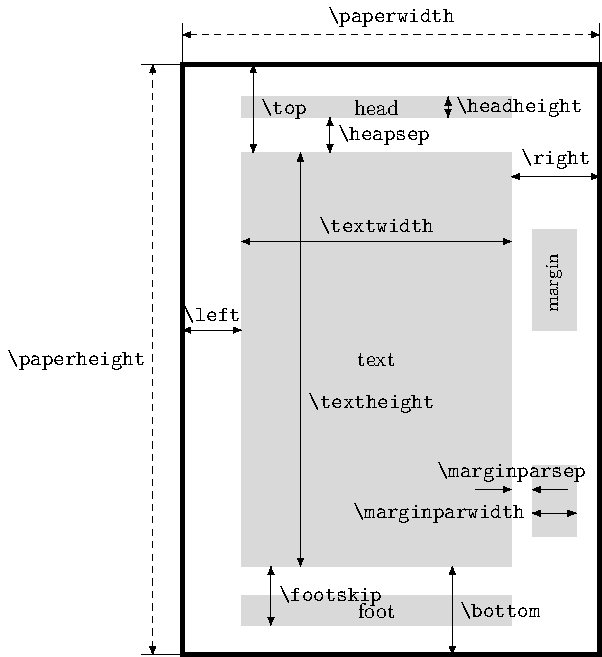
\includegraphics[scale=0.8]{./resource/tikz/geometry.pdf}

\end{tcolorbox}

\item 页面尺寸设置:\boxforpkg{geometry} 宏包提供了各种设置页面的工具,调整 {\tt paper=\ttit name} 选项可以设置纸张尺寸名,例如 \verb|a4paper|,\verb|ansibpaper|,\verb|letterpaper|,\verb|executivepaper|,\verb|legalpaper| 等。也可以通过 {\tt papersize=\{{\ttit width},{\ttit height}\}} 调整特定的纸张宽高,或用 {\tt paperwidth=\ttit size} 和 {\tt paperheight=\ttit size} 选项单独调整宽或高。

使用 \verb|landscape| 选项可以设置纸张为横向,默认是 \verb|portrait| 纵向。

\item 理解页面的元素:一个页面可以包含页眉(head)、页脚(foot)、侧边栏(margin note)和文本主体(body)这几个元素组成。这几个元素可以单独或共同构成总文本区(total body)。

使用 {\tt scale=\ttit scalar} 选项可以控制总文本区占纸张总尺寸的比例,默认为 0.7 。总文本区默认设置为 \verb|includehead| 表示包含页眉,可以使用 \verb|include| 或 \verb|ignore| 加上 \verb|foot| 、\verb|head| 、\verb|headfoot| 、\verb|mp| 、\verb|all| 构成的选项自由调节总文本区的组成,并使用 \verb|(total)?width=| 和 \verb|(total)?height=| 以及 {\tt total=\{{\ttit width},{\ttit height}\}} 调节总文本区的尺寸。

文本主体的尺寸由 \verb|textwidth=| 和 \verb|textheight=| 以及 {\tt body=\{{\ttit width},{\ttit height}\}} 调节。

页面边距 \verb|top left bottom right| 都是相对文本主体的边距。书籍相关的文档类一般都提供了 \verb|twoside| 选项,此时纸张两面相对书脊位置是相反的,因此有 \verb|inner=| 和 \verb|outer=| 左右边距的意义。可以用 \verb|hmargin=| 和 \verb|vmargin=| 指定水平和竖直的两边距,或者用 \verb|hmarginratio=| 指定水平左右或内外边距之比(默认为单页 1.0 和双页 0.67)以及 \verb|vmarginratio=| 指定竖直上下边距之比。使用 \verb|hcentering| 、\verb|vcentering| 或 \verb|centering| 可以使文本主体居中,从而使边距相等。在文档的左侧或内侧,可以使用 \verb|bindingoffset=| 预留装订线宽度。

页眉的高度使用 \verb|head(height)?=| 参数指定,侧边栏的宽度由 \verb|marginparwidth| 指定。页脚的高度主要由内容决定,也可以通过 \verb|foot(skip)?=| 设置最大高度。它们离文本主体的间距分别由参数 \verb|headsep| 、\verb|footnotesep| 、\verb|marginparsep| 指定。通过 \verb|nohead| 、\verb|nofoot| 、\verb|nomarginpar| 可以清除对应部分的所有尺寸,但不会删除内容。

总之,如果想查看页面元素的位置,可以通过 \verb|showframe| 选项给所有元素加上边框,便于检查尺寸。

\item 页面样式:使用 \boxforcmd{\\pagestyle{}} 可以设置页面样式。页面样式主要影响页眉和页脚。默认可用的页面样式有:

\begin{tcolorbox}[colback=white]
\centering
\begin{tabular}{ll}
    样式 & 效果 \\
\hline
    \verb|empty| & 无页眉页脚 \\
    \verb|plain| & 无页眉,页脚仅中央显示页码 \\
    \verb|headings| & 无页眉,页脚包含页码和章节名 \\
    \verb|myheadings| & 无页眉,页脚包含页码和自定义信息 \\
\end{tabular}
\end{tcolorbox}

使用 \boxforcmd{\\thispagestyle{}} 可以仅设置某一页样式。例如,可以将封面页设置为 \verb|empty| 样式。

\item 自定义页眉页脚:\boxforpkg{fancyhdr} 宏包提供了 \verb|fancy| 页面样式,可以自定义页眉页脚内容。使用 \verb|lcr| 和 \verb|head| 或 \verb|foot| 组成的各种命令如 \boxforcmd{\\rhead{}} 可以自定义页眉页脚的左中右内容。

\boxforpkg{fancyhdr} 宏包还可以修改页眉线和页脚线宽,需要通过 \lstinline|\renewcommand{\headrulewidth}{0.4pt}| 这种重定义命令的形式设置。

通过命令 \boxforcmd{\\thepage} 可以获取当前的页码数。以下是一个综合示例:

\begin{tcolorbox}[sidebyside]
\begin{lstlisting}
\usepackage{fancyhdr}
\pagestyle{fancy}
\lhead{Chapter 2}
% ...
\cfoot{page \thepage}
\rfoot{$e^{\pi i}+1=0$}
\renewcommand{\footrulewidth}{0.4pt}
\end{lstlisting}

\tcblower

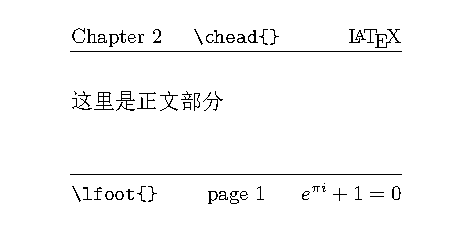
\includegraphics{./resource/tikz/hdr.pdf}
\end{tcolorbox}

使用 \boxforcmd{\\fancyhead[]{}} 和 \boxforcmd{\\fancyfoot[]{}} 可以解决书籍双页环境下的位置问题,该命令可选参数可以使用 \boxforcmd{EO} 和 \boxforcmd{LCR} 的组合表示位置,前者表示左页或右叶位置,后者表示左中右位置。


\item 多栏排版:
\begin{multicols}{2}
    
    使用文档类提供的 \verb|twocolumn| 可选参数项可以使文章变成两栏,默认为 \verb|onecolumn| 一栏。多栏文档的 \boxforcmd{\\newpage} 用于换栏,而 \boxforcmd{\\clearpage} 才是换页。
    
    排版过程中也可以使用 \boxforcmd{\\twocolumn} 或 \boxforcmd{onecolumn} 声明来切换单双栏,同时执行换页、清空浮动队列(即将图表等内容输出)。如果双栏命令带上了可选参数,则可选参数的内容将作为双栏上方的跨栏文本,一般用作双栏前的标题。这两个声明可以放在导言区或当前分组环境内。

    多栏下栏之间的间隔距离由 \verb|\columnsep| 给出;栏宽间隔和文本主题的宽度确定,由 \verb|\columnwidth| 给出。
    
    \vspace{1em}
    
    如果要局部分栏或使用任意多栏,可以使用 \boxforpkg{multicol} 宏包提供的 \boxforenv{multicols} 环境,它的完整环境参数为 \fbox{\tt\{multicols\}\{n\}[{\ttit preface}][{\ttit skip}]} 。一个额外的必选参数指定了分栏数,可以为 2--10 。可选参数 {\ttit preface} 指定多栏上方的跨栏文本(标题),另一个可选参数 {\ttit skip} 表示多栏环境的预留高度,如果当前文本区的内容小于该值,则系统将换页并从下一页开始排版它。但这个参数不影响多栏环境的实际高度。
   
    在 \boxforenv{multicols} 环境下,可以使用 \boxforcmd{\\columnbreak} 命令强制换栏。

    \boxforenv{multicols} 环境与文档类自带的双栏选项的区别在于,它追求最小的高度,因此左右两栏内容是等高的,左右两栏会自动调节内容。而文档类的双栏只有左栏排满后才转到右栏排版,两侧内容往往不相等。可以在 \boxforenv{multicols} 环境开始命令之前使用命令 \boxforcmd{\\raggedcolumns} 使每栏文本的底部可以不对齐,防止多栏的段落间距出问题。

\end{multicols}

\item 多栏排版的分隔线:多栏排版下栏之间的分隔线宽度由 \boxforcmdbox{\tt \textbackslash columnseprule={\ttit size}} 给出,它的默认值是 0pt ,因此默认不显示分隔线。

使用宏包 \boxforpkg{multicolrule} 可以设置各种样式的多栏分隔线。使用声明 \boxforcmd{\SetMCRule{line-style=...,width=...}} 可以修改分隔线,选项 \verb|line-style| 改变分隔线样式,可用值有 \verb|dots| 、\verb|circles| 、\verb|dotted| 、\verb|dash-dot| 、\verb|dashed| 等;选项 \verb|width=| 修改线宽,可以是 \verb|thin| 、\verb|thick| 、\verb|2pt| 等。

\item 侧边栏与边注:多栏排版有专用的命令,侧边栏一般用于编写简短的注解。

\hspace{-0.8cm}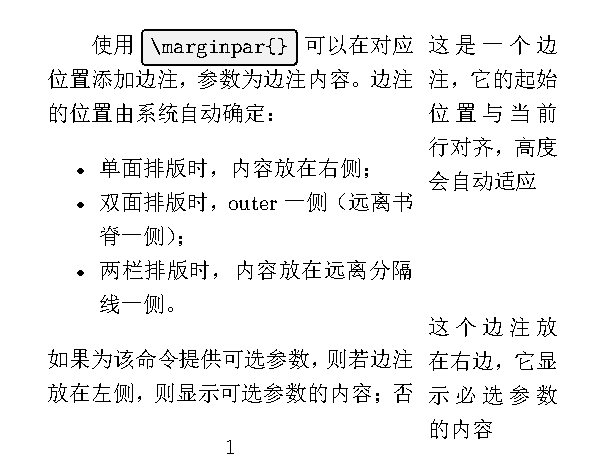
\includegraphics{./resource/tikz/margin-note-page1.pdf}\rule{0.3pt}{8cm}
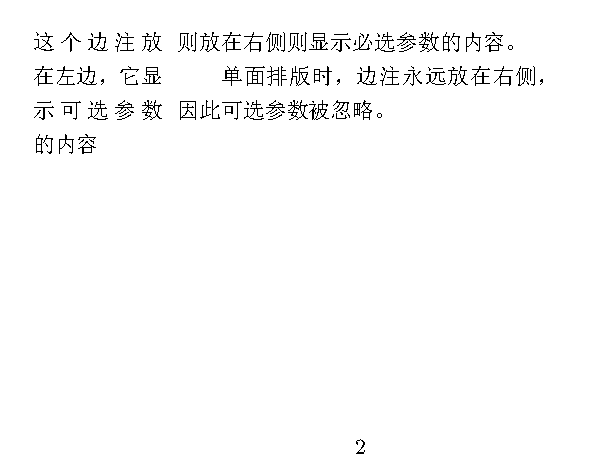
\includegraphics{./resource/tikz/margin-note-page2.pdf}

以上书籍文档类的效果,书籍的第一页通常都在右侧,它与双栏不同。

\item 脚注:

\hspace{-1.6cm}
\includegraphics{./resource/tikz/foot-note.pdf}



\end{enumerate}